% Model_LocalPolar.tex
% Face-on view of the lens plane, showing the local polar coordinate
% system (theta-tilde, phi) centred on the image, together with the
% global coordinate directions (theta_1, theta_2).
% Colour palette chosen at mid luminance so it stays legible on both
% white and black page backgrounds.
\documentclass[border=4pt]{standalone}
\usepackage{tikz}
\usepackage{amsmath}
\usetikzlibrary{arrows.meta, decorations.markings, calc}

\definecolor{inkcol}{RGB}{125,132,140}
\definecolor{planecol}{RGB}{155,155,155}
\definecolor{lenscol}{RGB}{215,135,45}
\definecolor{imgcol}{RGB}{205,165,45}
\definecolor{anglecol}{RGB}{170,95,200}

% the kidney/banana shaped blob used for the distorted lensed image
\tikzset{
  kidney/.pic={
    \fill[imgcol]
      (0,1) .. controls (0.55,0.95) and (1.0,0.4)  .. (1.0,0)
            .. controls (1.0,-0.4)  and (0.55,-0.95) .. (0,-1)
            .. controls (0.15,-0.75) and (0.35,-0.3) .. (0.35,0)
            .. controls (0.35,0.3)  and (0.15,0.75) .. cycle;
  }
}

\begin{document}
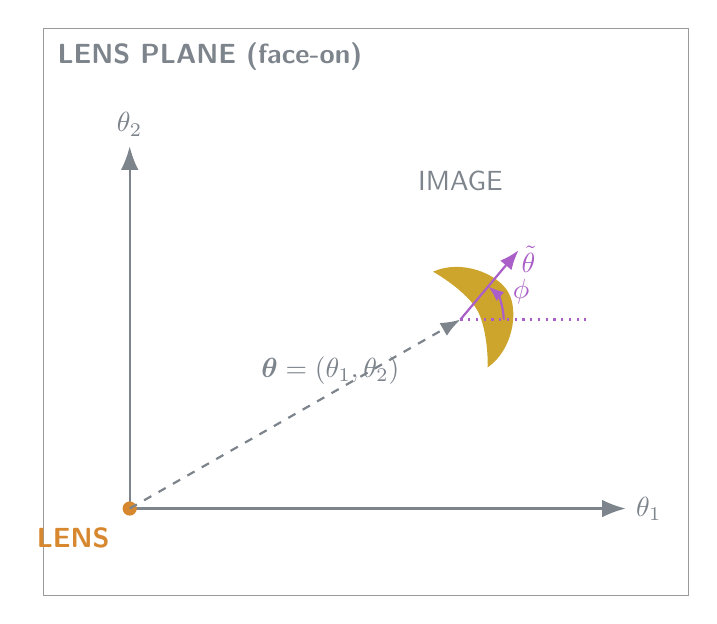
\begin{tikzpicture}[
    >=Latex,
    line width=1pt,
    font=\sffamily
  ]

  % --- coordinates -------------------------------------------------------
  \coordinate (Origin) at (0,0);
  \coordinate (ImgPos) at (4.2,2.4);

  % --- frame, representing the lens plane viewed face-on -----------------
  \draw[planecol, thin] (-1.1,-1.1) rectangle (7.1,6.1);
  \node[inkcol, font=\sffamily\bfseries, anchor=north west] at (-1.05,6.05) {LENS PLANE (face-on)};

  % --- global coordinate axes, centred on the lens ------------------------
  \draw[inkcol, thick, -{Latex[length=3mm]}] (Origin) -- (6.3,0) node[right, font=\sffamily] {$\theta_1$};
  \draw[inkcol, thick, -{Latex[length=3mm]}] (Origin) -- (0,4.6) node[above, font=\sffamily] {$\theta_2$};
  \fill[lenscol] (Origin) circle (0.09);
  \node[lenscol, font=\sffamily\bfseries, anchor=north east] at (-0.12,-0.12) {LENS};

  % --- position vector of the image, theta = (theta_1,theta_2) -----------
  \draw[inkcol, thick, dashed, -{Latex[length=2.5mm]}] (Origin) -- (ImgPos);
  \node[inkcol, font=\sffamily] at ($(Origin)+(2.55,1.75)$) {$\boldsymbol{\theta}=(\theta_1,\theta_2)$};

  % --- the image itself (kidney/banana shape), concave side facing the lens
  \pic[scale=0.7, rotate=29.74] at (ImgPos) {kidney};
  \node[inkcol, font=\sffamily, anchor=south] at ($(ImgPos)+(0,1.5)$) {IMAGE};

  % --- local polar axis (phi = 0 reference direction, parallel to theta_1)
  \draw[anglecol, dotted, thick] (ImgPos) -- ($(ImgPos)+(1.6,0)$);

  % --- radius theta-tilde, at a representative angle phi -----------------
  \draw[anglecol, thick, -{Latex[length=2.5mm]}]
    (ImgPos) -- ($(ImgPos)+(50:1.15)$);
  \node[anglecol, font=\sffamily, anchor=west] at ($(ImgPos)+(50:1.0)$) {$\tilde{\theta}$};

  % --- angle phi, measured from the local polar axis ----------------------
  \draw[anglecol, thick, -{Latex[length=2mm]}]
    ($(ImgPos)+(0:0.55)$) arc [start angle=0, end angle=50, radius=0.55];
  \node[anglecol, font=\sffamily] at ($(ImgPos)+(25:0.85)$) {$\phi$};

\end{tikzpicture}
\end{document}
